% Options for packages loaded elsewhere
\PassOptionsToPackage{unicode}{hyperref}
\PassOptionsToPackage{hyphens}{url}
%
\documentclass[
  ignorenonframetext,
]{beamer}
\usepackage{pgfpages}
\setbeamertemplate{caption}[numbered]
\setbeamertemplate{caption label separator}{: }
\setbeamercolor{caption name}{fg=normal text.fg}
\beamertemplatenavigationsymbolsempty
% Prevent slide breaks in the middle of a paragraph
\widowpenalties 1 10000
\raggedbottom
\setbeamertemplate{part page}{
  \centering
  \begin{beamercolorbox}[sep=16pt,center]{part title}
    \usebeamerfont{part title}\insertpart\par
  \end{beamercolorbox}
}
\setbeamertemplate{section page}{
  \centering
  \begin{beamercolorbox}[sep=12pt,center]{part title}
    \usebeamerfont{section title}\insertsection\par
  \end{beamercolorbox}
}
\setbeamertemplate{subsection page}{
  \centering
  \begin{beamercolorbox}[sep=8pt,center]{part title}
    \usebeamerfont{subsection title}\insertsubsection\par
  \end{beamercolorbox}
}
\AtBeginPart{
  \frame{\partpage}
}
\AtBeginSection{
  \ifbibliography
  \else
    \frame{\sectionpage}
  \fi
}
\AtBeginSubsection{
  \frame{\subsectionpage}
}
\usepackage{amsmath,amssymb}
\usepackage{iftex}
\ifPDFTeX
  \usepackage[T1]{fontenc}
  \usepackage[utf8]{inputenc}
  \usepackage{textcomp} % provide euro and other symbols
\else % if luatex or xetex
  \usepackage{unicode-math} % this also loads fontspec
  \defaultfontfeatures{Scale=MatchLowercase}
  \defaultfontfeatures[\rmfamily]{Ligatures=TeX,Scale=1}
\fi
\usepackage{lmodern}
\ifPDFTeX\else
  % xetex/luatex font selection
\fi
% Use upquote if available, for straight quotes in verbatim environments
\IfFileExists{upquote.sty}{\usepackage{upquote}}{}
\IfFileExists{microtype.sty}{% use microtype if available
  \usepackage[]{microtype}
  \UseMicrotypeSet[protrusion]{basicmath} % disable protrusion for tt fonts
}{}
\makeatletter
\@ifundefined{KOMAClassName}{% if non-KOMA class
  \IfFileExists{parskip.sty}{%
    \usepackage{parskip}
  }{% else
    \setlength{\parindent}{0pt}
    \setlength{\parskip}{6pt plus 2pt minus 1pt}}
}{% if KOMA class
  \KOMAoptions{parskip=half}}
\makeatother
\usepackage{xcolor}
\newif\ifbibliography
\usepackage{color}
\usepackage{fancyvrb}
\newcommand{\VerbBar}{|}
\newcommand{\VERB}{\Verb[commandchars=\\\{\}]}
\DefineVerbatimEnvironment{Highlighting}{Verbatim}{commandchars=\\\{\}}
% Add ',fontsize=\small' for more characters per line
\usepackage{framed}
\definecolor{shadecolor}{RGB}{248,248,248}
\newenvironment{Shaded}{\begin{snugshade}}{\end{snugshade}}
\newcommand{\AlertTok}[1]{\textcolor[rgb]{0.94,0.16,0.16}{#1}}
\newcommand{\AnnotationTok}[1]{\textcolor[rgb]{0.56,0.35,0.01}{\textbf{\textit{#1}}}}
\newcommand{\AttributeTok}[1]{\textcolor[rgb]{0.13,0.29,0.53}{#1}}
\newcommand{\BaseNTok}[1]{\textcolor[rgb]{0.00,0.00,0.81}{#1}}
\newcommand{\BuiltInTok}[1]{#1}
\newcommand{\CharTok}[1]{\textcolor[rgb]{0.31,0.60,0.02}{#1}}
\newcommand{\CommentTok}[1]{\textcolor[rgb]{0.56,0.35,0.01}{\textit{#1}}}
\newcommand{\CommentVarTok}[1]{\textcolor[rgb]{0.56,0.35,0.01}{\textbf{\textit{#1}}}}
\newcommand{\ConstantTok}[1]{\textcolor[rgb]{0.56,0.35,0.01}{#1}}
\newcommand{\ControlFlowTok}[1]{\textcolor[rgb]{0.13,0.29,0.53}{\textbf{#1}}}
\newcommand{\DataTypeTok}[1]{\textcolor[rgb]{0.13,0.29,0.53}{#1}}
\newcommand{\DecValTok}[1]{\textcolor[rgb]{0.00,0.00,0.81}{#1}}
\newcommand{\DocumentationTok}[1]{\textcolor[rgb]{0.56,0.35,0.01}{\textbf{\textit{#1}}}}
\newcommand{\ErrorTok}[1]{\textcolor[rgb]{0.64,0.00,0.00}{\textbf{#1}}}
\newcommand{\ExtensionTok}[1]{#1}
\newcommand{\FloatTok}[1]{\textcolor[rgb]{0.00,0.00,0.81}{#1}}
\newcommand{\FunctionTok}[1]{\textcolor[rgb]{0.13,0.29,0.53}{\textbf{#1}}}
\newcommand{\ImportTok}[1]{#1}
\newcommand{\InformationTok}[1]{\textcolor[rgb]{0.56,0.35,0.01}{\textbf{\textit{#1}}}}
\newcommand{\KeywordTok}[1]{\textcolor[rgb]{0.13,0.29,0.53}{\textbf{#1}}}
\newcommand{\NormalTok}[1]{#1}
\newcommand{\OperatorTok}[1]{\textcolor[rgb]{0.81,0.36,0.00}{\textbf{#1}}}
\newcommand{\OtherTok}[1]{\textcolor[rgb]{0.56,0.35,0.01}{#1}}
\newcommand{\PreprocessorTok}[1]{\textcolor[rgb]{0.56,0.35,0.01}{\textit{#1}}}
\newcommand{\RegionMarkerTok}[1]{#1}
\newcommand{\SpecialCharTok}[1]{\textcolor[rgb]{0.81,0.36,0.00}{\textbf{#1}}}
\newcommand{\SpecialStringTok}[1]{\textcolor[rgb]{0.31,0.60,0.02}{#1}}
\newcommand{\StringTok}[1]{\textcolor[rgb]{0.31,0.60,0.02}{#1}}
\newcommand{\VariableTok}[1]{\textcolor[rgb]{0.00,0.00,0.00}{#1}}
\newcommand{\VerbatimStringTok}[1]{\textcolor[rgb]{0.31,0.60,0.02}{#1}}
\newcommand{\WarningTok}[1]{\textcolor[rgb]{0.56,0.35,0.01}{\textbf{\textit{#1}}}}
\usepackage{longtable,booktabs,array}
\usepackage{calc} % for calculating minipage widths
\usepackage{caption}
% Make caption package work with longtable
\makeatletter
\def\fnum@table{\tablename~\thetable}
\makeatother
\usepackage{graphicx}
\makeatletter
\def\maxwidth{\ifdim\Gin@nat@width>\linewidth\linewidth\else\Gin@nat@width\fi}
\def\maxheight{\ifdim\Gin@nat@height>\textheight\textheight\else\Gin@nat@height\fi}
\makeatother
% Scale images if necessary, so that they will not overflow the page
% margins by default, and it is still possible to overwrite the defaults
% using explicit options in \includegraphics[width, height, ...]{}
\setkeys{Gin}{width=\maxwidth,height=\maxheight,keepaspectratio}
% Set default figure placement to htbp
\makeatletter
\def\fps@figure{htbp}
\makeatother
\setlength{\emergencystretch}{3em} % prevent overfull lines
\providecommand{\tightlist}{%
  \setlength{\itemsep}{0pt}\setlength{\parskip}{0pt}}
\setcounter{secnumdepth}{-\maxdimen} % remove section numbering
\ifLuaTeX
  \usepackage{selnolig}  % disable illegal ligatures
\fi
\IfFileExists{bookmark.sty}{\usepackage{bookmark}}{\usepackage{hyperref}}
\IfFileExists{xurl.sty}{\usepackage{xurl}}{} % add URL line breaks if available
\urlstyle{same}
\hypersetup{
  pdftitle={Module 2: MULTIPLE LINEAR REGRESSION Week 2},
  pdfauthor={Mette Langaas, Department of Mathematical Sciences, NTNU -- with contributions from Øyvind Bakke and Ingeborg Hem},
  hidelinks,
  pdfcreator={LaTeX via pandoc}}

\title{Module 2: MULTIPLE LINEAR REGRESSION Week 2}
\subtitle{TMA4315 Generalized linear models H2018}
\author{Mette Langaas, Department of Mathematical Sciences, NTNU -- with
contributions from Øyvind Bakke and Ingeborg Hem}
\date{30.08 and 06.09 {[}PL{]}, 31.08 and 07.09 {[}IL{]}}

\begin{document}
\frame{\titlepage}

\begin{frame}
\begin{block}{What to remember?}
\protect\hypertarget{what-to-remember}{}
Model: \[
{\bf Y}= X {\boldsymbol \beta}+\boldsymbol{\varepsilon}
\]

with full rank design matrix. And classical \emph{normal} linear
regression model when \[\varepsilon\sim N_n(\bf{0},\sigma^2\bf{I}).\]

Parameter of interest is \(\beta\) and \(\sigma^2\) is a nuisance.
Maximum likelihood estimator
\[ \hat\beta=({\bf X}^T{\bf X})^{-1} {\bf X}^T {\bf Y}\] has
distribution:
\(\hat{\beta}\sim N_{p}(\beta,\sigma^2({\bf X}^T{\bf X})^{-1})\).

Restricted maximum likelihood estimator for \({\boldsymbol \sigma}^2\):

\[
\hat{\sigma}^2=\frac{1}{n-p}({\bf Y}-{\bf X}\hat{\beta})^T({\bf Y}-{\bf X}\hat{\beta})=\frac{\text{SSE}}{n-p}
\]

with \(\frac{(n-p)\hat{\sigma}^2}{\sigma^2} \sim \chi^2_{n-p}\).
\end{block}
\end{frame}

\begin{frame}
Statistic for inference about \(\beta_j\), \(c_{jj}\) is diagonal
element \(j\) of \(({\bf X}^T{\bf X})^{-1}\).

\[
T_j=\frac{\hat{\beta}_j-\beta_j}{\sqrt{c_{jj}}\hat{\sigma}}\sim t_{n-p}
\]

This requires that \(\hat{\beta}_j\) and \(\hat{\sigma}\) are
independent.
\end{frame}

\begin{frame}{Inference}
\protect\hypertarget{inference}{}
We will consider confidence intervals and prediction intervals, and then
test single and linear hypotheses.
\end{frame}

\begin{frame}
\begin{block}{Confidence intervals (CI)}
\protect\hypertarget{confidence-intervals-ci}{}
In addition to providing a parameter estimate for each element of our
parameter vector \(\beta\) we should also report a \((1-\alpha)100\)\%
confidence interval (CI) for each element. (We will not consider
simultanious confidence regions in this course.)

We focus on element \(j\) of \(\beta\), called \(\beta_j\). It is known
that \(T_j =\frac{\hat{\beta}_j-\beta_j}{\sqrt{c_{jj}}\hat{\sigma}}\)
follows a \(t\)-distribution with \(n-p\) degrees of freedom. Let
\(t_{\alpha/2,n-p}\) be such that \(P(T_j>t_{\alpha/2,n-p})=\alpha/2\).

Since the \(t\)-distribution is symmetric around 0, then
\(P(T_j< -t_{\alpha/2,n-p})=\alpha/2\). We may then write
\[P(-t_{\alpha/2,n-p}\le T_j \le t_{\alpha/2,n-p})=1-\alpha\]
\end{block}
\end{frame}

\begin{frame}
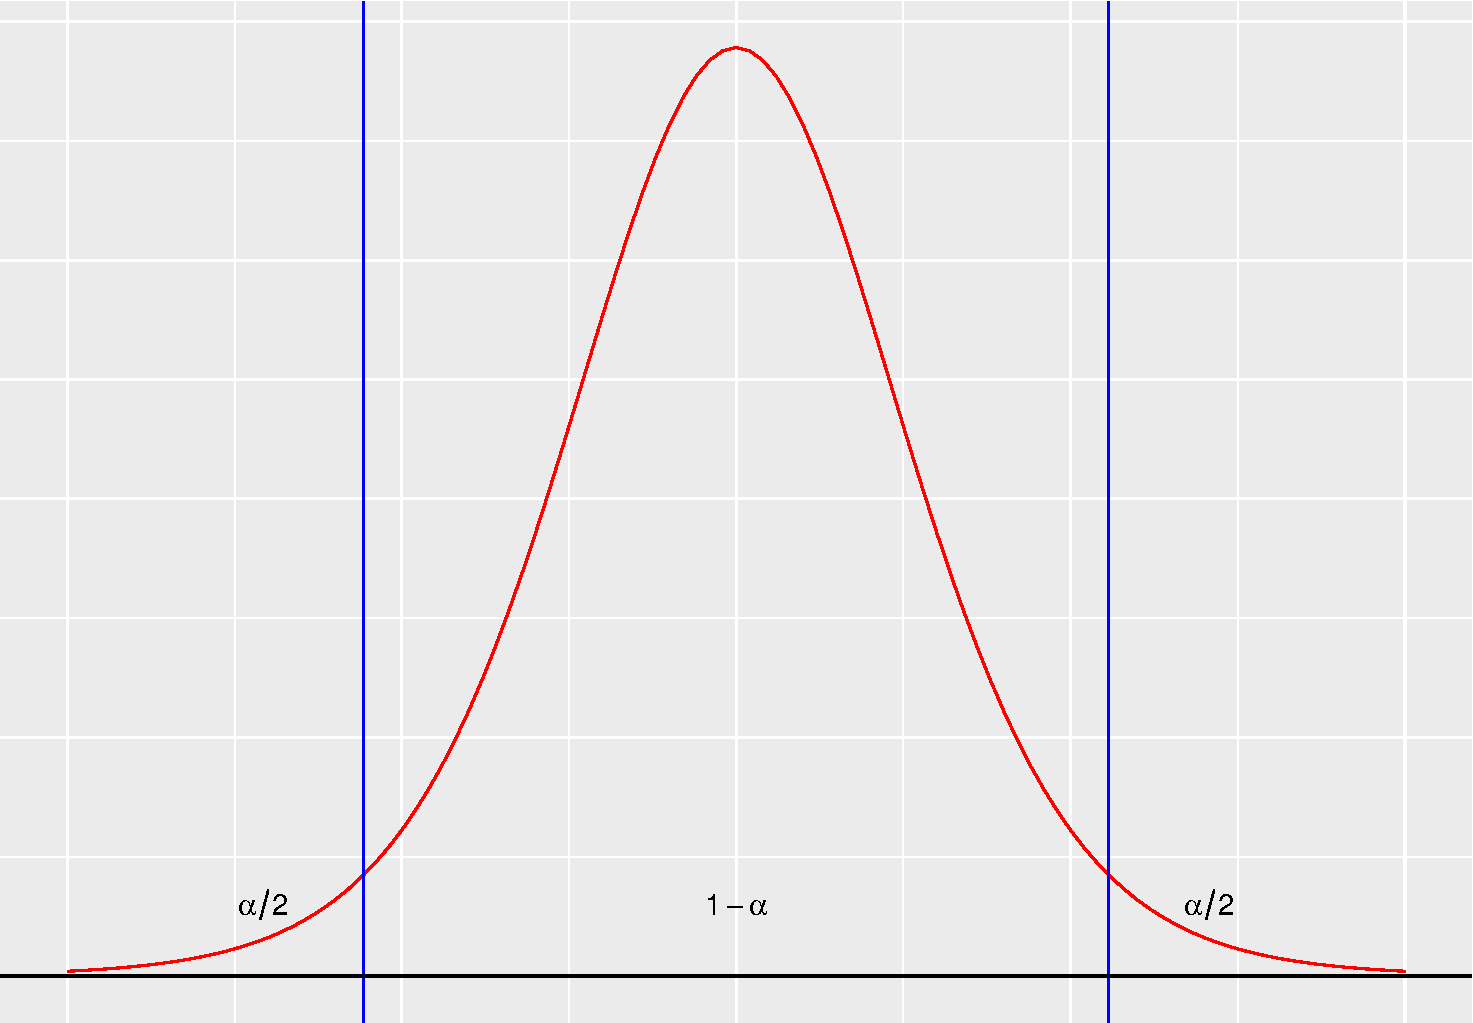
\includegraphics{Module02MLRPresentationWeek2_files/figure-beamer/unnamed-chunk-2-1.pdf}

(Blue lines at \(\pm t_{\alpha/2,n-p}\).)
\end{frame}

\begin{frame}
Inserting
\(T_j =\frac{\hat{\beta}_j-\beta_j}{\sqrt{c_{jj}}\hat{\sigma}}\) and
solving so \(\beta_j\) is in the middle gives:

\[ P(\hat{\beta}_j-t_{\alpha/2,n-p}\sqrt{c_{jj}}\hat{\sigma}
\le \beta_j \le \hat{\beta}_j+t_{\alpha/2,n-p}\sqrt{c_{jj}}\hat{\sigma})=1-\alpha\]

A \((1-\alpha)\)\% CI for \(\beta_j\) is when we insert numerical values
for the upper and lower limits:
\([\hat{\beta}_j-t_{\alpha/2,n-p}\sqrt{c_{jj}}\hat{\sigma},\hat{\beta}_j+t_{\alpha/2,n-p}\sqrt{c_{jj}}\hat{\sigma}]\).
\end{frame}

\begin{frame}[fragile]
CIs can be found in R using \texttt{confint} on an \texttt{lm} object.
(Here dummy variable coding is used for \texttt{location}, with average
as reference location.)

\begin{Shaded}
\begin{Highlighting}[]
\FunctionTok{library}\NormalTok{(gamlss.data)}
\NormalTok{fit }\OtherTok{=} \FunctionTok{lm}\NormalTok{(rent }\SpecialCharTok{\textasciitilde{}}\NormalTok{ area }\SpecialCharTok{+}\NormalTok{ location }\SpecialCharTok{+}\NormalTok{ bath }\SpecialCharTok{+}\NormalTok{ kitchen }\SpecialCharTok{+}\NormalTok{ cheating, }\AttributeTok{data =}\NormalTok{ rent99)}
\FunctionTok{confint}\NormalTok{(fit)}
\end{Highlighting}
\end{Shaded}

\begin{verbatim}
##                  2.5 %      97.5 %
## (Intercept) -44.825534   0.8788739
## area          4.354674   4.8029443
## location2    28.579849  49.9405909
## location3    92.970636 159.1443278
## bath1        52.076412  96.0311030
## kitchen1     94.907671 145.9621578
## cheating1   144.427555 178.4000215
\end{verbatim}
\end{frame}

\begin{frame}
\begin{block}{Prediction intervals}
\protect\hypertarget{prediction-intervals}{}
Remember, one aim for regression was to ``construct a model to predict
the reponse from a set of (one or several) explanatory variables- more
or less black box''.

Assume we want to make a prediction (of the response - often called
\(Y_0\)) given specific values for the covariates - often called
\({\bf x}_0\). An intuitive point estimate is
\(\hat{Y}_0={\bf x}_0^T \hat{\beta}\) - but to give a hint of the
uncertainty in this prediction we also want to present a prediction
interval for the \(Y_0\).
\end{block}
\end{frame}

\begin{frame}
First, we assume that the unobserved response at covariate \({\bf x}_0\)
is independent of our previous observations and follows the same
distribution, that is \(Y_0 \sim N({\bf x}_0^T \beta,\sigma^2)\).
Further,

\[\hat{Y}_0={\bf x}_0^T \hat{\beta} \sim N({\bf x}_0^T \beta,\sigma^2 {\bf x}_0^T({\bf X}^T{\bf X})^{-1}{\bf x}_0).\]

Then, for \(Y_0-{\bf x}_0^T \hat{\beta}\) we have
\[\text{E}(Y_0-{\bf x}_0^T \hat{\beta})=0 \text{ and } \text{Var}(Y_0-{\bf x}_0^T \hat{\beta})=\text{Var}(Y_0)+\text{Var}({\bf x}_0^T \hat{\beta})=\sigma^2+\sigma^2{\bf x}_0^T({\bf X}^T{\bf X})^{-1}{\bf x}_0\]
so that
\[Y_0-{\bf x}_0^T \hat{\beta}\sim N(0,\sigma^2 (1+{\bf x}_0^T({\bf X}^T{\bf X})^{-1}{\bf x}_0)) \]
Inserting our REML-estimate for \(\sigma^2\) gives

\[T=\frac{Y_0-{\bf x}_0^T \hat{\beta}}{\hat{\sigma}\sqrt{1+{\bf x}_0^T({\bf X}^T{\bf X})^{-1}{\bf x}_0}}\sim t_{n-p}.\]
\end{frame}

\begin{frame}
Then, we start with
\[ P(-t_{\alpha/2,n-p}\le \frac{Y_0-{\bf x}_0^T \hat{\beta}}{\hat{\sigma}\sqrt{1+{\bf x}_0^T({\bf X}^T{\bf X})^{-1}{\bf x}_0}} \le t_{\alpha/2,n-p})=1-\alpha\]
and solve so that \(Y_0\) is in the middle, which gives
\[P({\bf x}_0^T \hat{\beta}-t_{\alpha/2,n-p}\hat{\sigma}\sqrt{1+{\bf x}_0^T({\bf X}^T{\bf X})^{-1}{\bf x}_0} \le Y_0 \le {\bf x}_0^T \hat{\beta}+t_{\alpha/2,n-p}\hat{\sigma}\sqrt{1+{\bf x}_0^T({\bf X}^T{\bf X})^{-1}{\bf x}_0})=1-\alpha\]

A \((1-\alpha)\)\% PI for \(Y_0\) is when we insert numerical values for
the upper and lower limits:
\([{\bf x}_0^T \hat{\beta}-t_{\alpha/2,n-p}\hat{\sigma}\sqrt{1+{\bf x}_0^T({\bf X}^T{\bf X})^{-1}{\bf x}_0}, {\bf x}_0^T \hat{\beta}+t_{\alpha/2,n-p}\hat{\sigma}\sqrt{1+{\bf x}_0^T({\bf X}^T{\bf X})^{-1}{\bf x}_0}]\).
\end{frame}

\begin{frame}[fragile]
PIs can be found in R using \texttt{predict} on an \texttt{lm} object,
but make sure that \texttt{newdata} is a \texttt{data.frame} with the
same names as the original data.

We want to predict the rent - with PI - for an apartment with area 50
\(m^2\), location 2 (``good''), nice bath and kitchen and with central
heating:

\begin{Shaded}
\begin{Highlighting}[]
\FunctionTok{library}\NormalTok{(gamlss.data)}
\NormalTok{fit }\OtherTok{=} \FunctionTok{lm}\NormalTok{(rent }\SpecialCharTok{\textasciitilde{}}\NormalTok{ area }\SpecialCharTok{+}\NormalTok{ location }\SpecialCharTok{+}\NormalTok{ bath }\SpecialCharTok{+}\NormalTok{ kitchen }\SpecialCharTok{+}\NormalTok{ cheating, }\AttributeTok{data =}\NormalTok{ rent99)}
\NormalTok{newobs }\OtherTok{=}\NormalTok{ rent99[}\DecValTok{1}\NormalTok{, ]}
\NormalTok{newobs[}\DecValTok{1}\NormalTok{, ] }\OtherTok{=} \FunctionTok{c}\NormalTok{(}\ConstantTok{NA}\NormalTok{, }\ConstantTok{NA}\NormalTok{, }\DecValTok{50}\NormalTok{, }\ConstantTok{NA}\NormalTok{, }\DecValTok{2}\NormalTok{, }\DecValTok{1}\NormalTok{, }\DecValTok{1}\NormalTok{, }\DecValTok{1}\NormalTok{, }\ConstantTok{NA}\NormalTok{)}
\FunctionTok{predict}\NormalTok{(fit, }\AttributeTok{newdata =}\NormalTok{ newobs, }\AttributeTok{interval =} \StringTok{"prediction"}\NormalTok{, }\AttributeTok{type =} \StringTok{"response"}\NormalTok{)}
\end{Highlighting}
\end{Shaded}

\begin{verbatim}
##        fit      lwr      upr
## 1 602.1298 315.5353 888.7243
\end{verbatim}
\end{frame}

\begin{frame}[fragile]
\begin{block}{Questions:}
\protect\hypertarget{questions}{}
\begin{enumerate}
\item
  {When is a prediction interval of interest? }
\item
  {Explain the result from \texttt{predict} above. What are
  \texttt{fit}, \texttt{lwr}, \texttt{upr}?}
\item
  {What is the interpretation of a 95\% prediction interval? }
\end{enumerate}
\end{block}
\end{frame}

\begin{frame}
\begin{block}{Single hypothesis testing set-up}
\protect\hypertarget{single-hypothesis-testing-set-up}{}
In single hypothesis testing we are interesting in testing one null
hypothesis against an alternative hypothesis. In linear regression the
hypothesis is often about a regression parameter \(\beta_j\):
\[H_0: \beta_j=0 \text{ vs. } H_1: \beta_j\neq 0\]

Remark: we implicitly say that our test is done given that the other
variables are present in the model, that is, the other \(\beta_i\)s
(\(j\neq i\)) are not zero.
\end{block}
\end{frame}

\begin{frame}
\begin{block}{Two types of errors:}
\protect\hypertarget{two-types-of-errors}{}
\begin{itemize}
\item
  ``Reject \(H_0\) when \(H_0\) is true''=``false positives'' = ``type I
  error'' =``miscarriage of justice''. These are our \emph{fake news},
  which are very important for us to avoid.
\item
  ``Fail to reject \(H_0\) when \(H_1\) is true (and \(H_0\) is
  false)''=``false negatives'' = ``type II error''= ``guilty criminal go
  free''.
\end{itemize}
\end{block}
\end{frame}

\begin{frame}
We choose to reject \(H_0\) at some significance level \(\alpha\) if the
\(p\)-value of the test (see below) is smaller than the chosen
significance level. We say that : Type I error is ``controlled'' at
significance level \(\alpha\), which means that the probability of
miscarriage of justice (Type I error) does not exceed \(\alpha\).

\textbf{Q}: Draw a 2 by 2 table showing the connection between

\begin{itemize}
\tightlist
\item
  ``truth'' (\(H_0\) true or \(H_0\) false) - rows in the table, and
\item
  ``action'' (reject \(H_0\) and accept \(H_0\)) - columns in the table,
\end{itemize}

and place the two types of errors in the correct position within the
table.

What else should be written in the last two cells?
\end{frame}

\begin{frame}
\begin{block}{Hypothesis test on \(\beta_j\) (t-test)}
\protect\hypertarget{hypothesis-test-on-beta_j-t-test}{}
In linear regression models our test statistic for testing
\(H_0: \beta_j=0\) is
\[T_0=\frac{\hat{\beta}_j-0}{\sqrt{c_{jj}}\hat{\sigma}_{\varepsilon}}\sim t_{n-2}\]
where
\(c_{jj}\hat{\sigma}_{\varepsilon}^2=\widehat{\text{Var}}(\hat{\beta}_j)\).

Inserted observed values (and estimates) we have \(t_0\).

We would in a two-sided setting reject \(H_0\) for large values of
\(\text{abs}(t_0)\). We may rely on calculating a \(p\)-value.
\end{block}
\end{frame}

\begin{frame}
\begin{block}{The p-value}
\protect\hypertarget{the-p-value}{}
A p-value is a test statistic satisfying \(0 \leq p({\bf Y}) \leq 1\)
for every vector of observations \({\bf Y}\).

\begin{itemize}
\item
  Small values are interpreted as evidence that \(H_1\) is true(-ish).
\item
  In single hypothesis testing, if the p-value is less than the chosen
  significance level (chosen upper limit for the probability of
  committing a type I error), then we reject the null hypothesis,
  \(H_0\). The chosen significance level is often referred to as
  \(\alpha\).
\item
  A p-value is \emph{valid} if
  \[ P(p({\bf Y}) \leq \alpha) \leq \alpha\] for all \(\alpha\),
  \(0 \leq \alpha \leq 1\), whenever \(H_0\) is true, that is, if the
  \(p\)-value is valid, rejection on the basis of the \(p\)-value
  ensures that the probability of type I error does not exceed
  \(\alpha\).
\item
  If \(P(p({\bf Y}) \leq \alpha) = \alpha\) for all \(\alpha\),
  \(0 \leq \alpha \leq 1\), the \(p\)-value is called an \emph{exact}
  p-value.
\end{itemize}
\end{block}
\end{frame}

\begin{frame}
In our linear regression we use the \(t\)-distibution to calculate
p-values for our two-sided test situation \(H_0: \beta_j=0\)
vs.~\(H_1: \beta_j \neq 0\). Assume we have observed that our test
statistic \(T_0\) takes the numerical value \(t_0\). Since the
\(t\)-distribution is symmetric around \(0\) we have

\[p\text{-value}=P(T_0>\text{abs}(t_0))+P(T_0<-\text{abs}(t_0))=2\cdot P(T_0>\text{abs}(t_0)).\]

We reject \(H_0\) if our calculated \(p\)-value is below our chosen
signficance level. We often choose as significance level
\(\alpha=0.05\).
\end{frame}

\begin{frame}[fragile]
\begin{block}{Munich rent index hypothesis test}
\protect\hypertarget{munich-rent-index-hypothesis-test}{}
We look at print-out using \texttt{summary} from fitting \texttt{lm}.

\begin{Shaded}
\begin{Highlighting}[]
\FunctionTok{library}\NormalTok{(gamlss.data)}
\NormalTok{fit }\OtherTok{=} \FunctionTok{lm}\NormalTok{(rent }\SpecialCharTok{\textasciitilde{}}\NormalTok{ area }\SpecialCharTok{+}\NormalTok{ location }\SpecialCharTok{+}\NormalTok{ bath }\SpecialCharTok{+}\NormalTok{ kitchen }\SpecialCharTok{+}\NormalTok{ cheating, }\AttributeTok{data =}\NormalTok{ rent99)}
\NormalTok{knitr}\SpecialCharTok{::}\FunctionTok{kable}\NormalTok{(}\FunctionTok{summary}\NormalTok{(fit)}\SpecialCharTok{$}\NormalTok{coefficients, }\AttributeTok{digits =} \DecValTok{3}\NormalTok{)}
\end{Highlighting}
\end{Shaded}

\begin{longtable}[]{@{}lrrrr@{}}
\toprule\noalign{}
& Estimate & Std. Error & t value &
Pr(\textgreater\textbar t\textbar) \\
\midrule\noalign{}
\endhead
(Intercept) & -21.973 & 11.655 & -1.885 & 0.059 \\
area & 4.579 & 0.114 & 40.055 & 0.000 \\
location2 & 39.260 & 5.447 & 7.208 & 0.000 \\
location3 & 126.057 & 16.875 & 7.470 & 0.000 \\
bath1 & 74.054 & 11.209 & 6.607 & 0.000 \\
kitchen1 & 120.435 & 13.019 & 9.251 & 0.000 \\
cheating1 & 161.414 & 8.663 & 18.632 & 0.000 \\
\bottomrule\noalign{}
\end{longtable}
\end{block}
\end{frame}

\begin{frame}[fragile]
\textbf{Q} (and A):

\begin{enumerate}
\item
  Where is hypothesis testing performed here, and which are the
  hypotheses rejected at level \(0.01\)?
\item
  Will the test statistics and \(p\)-values change if we change the
  regression model?
\item
  What is the relationship between performing an hypothesis test and
  constructing a CI interval? Remember:
\end{enumerate}

\begin{Shaded}
\begin{Highlighting}[]
\FunctionTok{library}\NormalTok{(gamlss.data)}
\NormalTok{fit }\OtherTok{=} \FunctionTok{lm}\NormalTok{(rent }\SpecialCharTok{\textasciitilde{}}\NormalTok{ area }\SpecialCharTok{+}\NormalTok{ location }\SpecialCharTok{+}\NormalTok{ bath }\SpecialCharTok{+}\NormalTok{ kitchen }\SpecialCharTok{+}\NormalTok{ cheating, }\AttributeTok{data =}\NormalTok{ rent99)}
\FunctionTok{confint}\NormalTok{(fit)}
\end{Highlighting}
\end{Shaded}

\begin{verbatim}
##                  2.5 %      97.5 %
## (Intercept) -44.825534   0.8788739
## area          4.354674   4.8029443
## location2    28.579849  49.9405909
## location3    92.970636 159.1443278
## bath1        52.076412  96.0311030
## kitchen1     94.907671 145.9621578
## cheating1   144.427555 178.4000215
\end{verbatim}
\end{frame}

\begin{frame}
\begin{block}{Testing linear hypotheses in regression}
\protect\hypertarget{testing-linear-hypotheses-in-regression}{}
We study a normal linear regression model with \(p=k+1\) covariates, and
refer to this as model A (the larger model). We then want to investigate
the null and alternative hypotheses of the following type(s):
\begin{eqnarray*}
 H_0: \beta_{j}&=&0 \text{ vs. } H_1:\beta_j\neq 0\\
 H_0: \beta_{1}&=&\beta_{2}=\beta_{3}=0 \text{ vs. } H_1:\text{ at least one of these }\neq 0\\
 H_0: \beta_{1}&=&\beta_{2}=\cdots=\beta_{k}=0 \text{ vs. } H_1:\text{ at least one of these }\neq 0\\
 \end{eqnarray*} We call the restricted model (when the null hypotesis
is true) model B, or the smaller model.
\end{block}
\end{frame}

\begin{frame}
These null hypotheses and alternative hypotheses can all be rewritten as
a linear hypothesis

\[
H_0: {\bf C}{\boldsymbol \beta}={\bf d} \text{ vs. } {\bf C}{\boldsymbol \beta}\neq {\bf d}
\]

by specifying \({\bf C}\) to be a \(r \times p\) matrix and \({\bf d}\)
to be a column vector of length \(p\).

The test statistic for performing the test is called \(F_{obs}\) and can
be formulated in two ways: \begin{eqnarray}
F_{obs}&=&\frac{\frac{1}{r} (SSE_{H_0}-SSE)}{\frac{SSE}{n-p}} \label{Fobsnested}\\
F_{obs}&=&\frac{1}{r}({\bf C}\hat{{\boldsymbol \beta}}-{\bf d})^{\text T}[\hat{\sigma}^2 {\bf C}({\bf X}^{\text T}{\bf X})^{-1}{\bf C}^{\text T}]^{-1}({\bf C}\hat{{\boldsymbol \beta}}-{\bf d}) \label{FobsCbeta}
\end{eqnarray} where \(SSE\) is from the larger model A, \(SSE_{H_0}\)
from the smaller model B, and \(\hat{{\boldsymbol \beta}}\) and
\(\hat{\sigma}^2\) are estimators from the larger model A.
\end{frame}

\begin{frame}
\begin{block}{Testing a set of parameters - what is \({\bf C}\) and
\({\bf d}\)?}
\protect\hypertarget{testing-a-set-of-parameters---what-is-bf-c-and-bf-d}{}
We consider a regression model with intercept and five covariates,
\(x_1, \ldots, x_5\). Assume that we want to know if the covariates
\(x_3\), \(x_4\), and \(x_5\) can be dropped (due to the fact that none
of the corresponding \(\beta_j\)s are different from zero). This means
that we want to test:

\[H_0: \beta_{3}=\beta_{4}=\beta_{5}=0 \text{ vs. } H_1:\text{ at least one of these }\neq 0\]
This means that our \({\bf C}\) is a \(6\times 3\) matrix and
\({\bf d}\) a \(3 \times 1\) column vector
\[ {\bf C}=\begin{pmatrix} 0 &0 &0 &1 &0&0 \\
0&0&0&0&1&0\\
0&0&0&0&0& 1\\
\end{pmatrix} \text{ and } 
{\bf d} \begin{pmatrix} 0\\0\\0\\ \end{pmatrix}\]
\end{block}
\end{frame}

\begin{frame}
\begin{block}{Testing one regression parameter}
\protect\hypertarget{testing-one-regression-parameter}{}
If we set \({\bf C}=(0,1, 0, \cdots, 0)^T\), a row vector with 1 in
position 2 and 0 elsewhere, and \({\bf d}=(0,0,\ldots,0)\), a column
vector with 0s, then we test
\[ H_0: \beta_1=0 \text{ vs. } H_1: \beta_1\neq 0.\] Now
\({\bf C}\hat{\beta}=\beta_1\) and
\({\bf C}({\bf X}^{\text T}{\bf X})^{-1}{\bf C}^{\text T}=c_{11}\), so
that \(F_{obs}\) then is equal to the square of the \(t\)-statistics for
testing a single regression parameter.
\[F_{obs}=(\hat{\beta}_1-0)^T[\hat{\sigma}^2 c_{jj}]^{-1}(\hat{\beta}_1-0)=T_1^2\]

Repeat the argument with \(\beta_j\) instead of \(\beta_1\).

Remark: Remember that \(T_{\nu}^2=F_{1,\nu}\).
\end{block}
\end{frame}

\begin{frame}
\begin{block}{Testing ``significance of the regression''}
\protect\hypertarget{testing-significance-of-the-regression}{}
If we set \({\bf C}=(0,1,1, \cdots ,1)^T\), a row vector with 0 in
position 1 and 0 elsewhere, and \({\bf d}=(0,0,\ldots,0)\), a column
vector with 0s, then we test
\[ H_0: \beta_1=\beta_2=\cdots= \beta_k =0 \text{ vs. } H_1: \text{at least one different from zero}.\]
This means we test if at least one of the regression parameters (in
addition to the intercept) is different from 0. The small model is then
the model with only the intercept, and for this model the SSE\(_{H_0}\)
is equal to SST (sums of squares total, see below). Let SSE be the
sums-of-squares of errors for the full model. If we have \(k\)
regression parameters (in addition to the intercept) then the
F-statistic becomes
\[ F_{obs}=\frac{\frac{1}{k}(\text{SST}-\text{SSE})}{\frac{\text{SSE}}{n-p}}\]
with \(k\) and \(n-p\) degrees of freedom under \(H_0\).
\end{block}
\end{frame}

\begin{frame}[fragile]
Is the regression significant?

\begin{Shaded}
\begin{Highlighting}[]
\FunctionTok{summary}\NormalTok{(fit)}\SpecialCharTok{$}\NormalTok{fstatistic}
\end{Highlighting}
\end{Shaded}

\begin{verbatim}
##     value     numdf     dendf 
##  420.0427    6.0000 3075.0000
\end{verbatim}
\end{frame}

\begin{frame}
\begin{block}{Relation to Wald test}
\protect\hypertarget{relation-to-wald-test}{}
Since \(\text{Cov}(\hat{\beta})=\sigma^2 ({\bf X}^T{\bf X})^{-1}\), then
\(\text{Cov}({\bf C}\hat{\beta})={\bf C}\sigma^2({\bf X}^T{\bf X})^{-1}{\bf C}^T\),
so that \({\bf C}\hat{\sigma}^2({\bf X}^T{\bf X})^{-1}{\bf C}^T\) can be
seen as an estimate of \(\text{Cov}({\bf C}\hat{\beta})\). Therefore,
\(F_{obs}\) can be written

\[F_{obs}=\frac{1}{r}({\bf C}\hat{{\bf \beta}}-{\bf d})^{\text T}[\widehat{\text{Cov}}({\bf C}\hat{\beta})]^{-1}({\bf C}\hat{{\bf \beta}}-{\bf d})=\frac{1}{r}W\]
where \(W\) is a so-called Wald test. It is known that
\(W\sim \chi^2_r\) asymptotically as \(n\) becomes large. We will study
the Wald test in more detail later in this course.
\end{block}
\end{frame}

\begin{frame}
\begin{block}{Asympotic result}
\protect\hypertarget{asympotic-result}{}
It can in general be shown that
\[r F_{r,n-p}\stackrel{n\rightarrow \infty}{\longrightarrow} \chi^2_r.\]
That is, if we have a random variable \(F\) that is distributed as
Fisher with \(r\) (numerator) and \(n-p\) (denominator) degrees of
freedom, then when \(n\) goes to infinity (\(p\) kept fixed), then
\(rF\) is approximately \(\chi^2\)-distributed with \(r\) degrees of
freedom.

Also, if our error terms are not normally distributed then we can assume
that when the number of observation becomes very large then
\(rF_{r,n-p}\) is approximately \(\chi^2_r\).
\end{block}
\end{frame}

\begin{frame}{Focus on likelihood: Likelihood ratio test and deviance}
\protect\hypertarget{focus-on-likelihood-likelihood-ratio-test-and-deviance}{}
\begin{block}{The likelihood ratio test}
\protect\hypertarget{the-likelihood-ratio-test}{}
An alternative to the Wald test is the likelihood ratio test (LRT),
which compares the likelihood of \emph{two models}.

We use the following notation. A: the larger model and B: the smaller
model (under \(H_0\)), and the smaller model is nested within the larger
model (that is, B is a submodel of A).
\end{block}
\end{frame}

\begin{frame}
\begin{itemize}
\tightlist
\item
  First we maximize the likelihood for model A (the larger model) and
  find the parameter estimate \(\hat{\beta}_A\). The maximum likelihood
  is achieved at this parameter estimate and is denoted
  \(L(\hat{\beta}_A)\).
\item
  Then we maximize the likelihood for model B (the smaller model) and
  find the parameter estimate \(\hat{\beta}_B\). The maximum likelihood
  is achieved at this parameter estimate and is denoted
  \(L(\hat{\beta}_B)\).
\end{itemize}

The likelihood of the larger model (A) will always be larger or equal to
the likelihood of the smaller model (B). Why?
\end{frame}

\begin{frame}
The likelihood ratio statistic is defined as
\[- 2\ln \lambda=-2(\ln L(\hat{\beta}_B)-\ln L(\hat{\beta}_A)) \] (so,
\(-2\) times small minus large).

Under weak regularity conditions the test statistic is approximately
\(\chi^2\)-distributed with degrees of freedom equal the difference in
the number of parameters in the large and the small model. This is
general - and not related to the GLM! More in TMA4295 Statistical
Inference!

\(P\)-values are calculated in the upper tail of the
\(\chi^2\)-distribution.

Observe: to perform the test you need to fit both the small and the
large model.
\end{frame}

\begin{frame}[fragile]
Notice: asymptotically the Wald and likelihood ratio test statistics
have the same distribution, but the value of the test statistics might
be different.

\begin{Shaded}
\begin{Highlighting}[]
\CommentTok{\# TRY OUT BOTH Wald and LRT}
\end{Highlighting}
\end{Shaded}

The LRT can be performed using \texttt{anova()}.
\end{frame}

\begin{frame}
\begin{block}{Deviance (something new!)}
\protect\hypertarget{deviance-something-new}{}
The \emph{deviance} is used to assess model fit and also for model
choice, and is based on the likelihood ratio test statistic. It is used
for all GLMs in general - and replaces using SSE in multiple linear
regression.

\textbf{Saturated model:} If we were to provide a perfect fit to our
data t

This ``imaginary model'' is called the \emph{saturated} model. This
would be a model where each observation was given its own parameter.

\textbf{Candidate model:} The model that we are investigated can be
thought of as a \emph{candidate} model. Then we maximize the likelihood
and get \(\hat{\beta}\).
\end{block}
\end{frame}

\begin{frame}
The \emph{deviance} is then defined as the likelihood ratio statistic,
where we put the saturated model in place of the larger model A and our
candidate model in place of the smaller model B:

\[D=-2(\ln L(\text{candidate model})-\ln L(\text{saturated model}))\]

For the maximal model, we have parameters \(\theta_1, \dots, \theta_n\),
where \(\theta_i = E[Y_i]\) The log-likelihood for this model is \[
l(\hat{\beta},{\sigma^2})=-\frac{n}{2}\text{ln}(2\pi)-\frac{n}{2}\text{ln}\sigma^2-\frac{1}{2\sigma^2} ({\bf y}-{\boldsymbol \theta})^T({\bf y}-{\boldsymbol \theta}) = -\frac{n}{2}\text{ln}(2\pi)-\frac{n}{2}\text{ln}\sigma^2
\]

(because \(\hat{\theta_i}=y_i\), something you may work out for
yourselves)
\end{frame}

\begin{frame}
The deviance is then

\[
\begin{aligned}
D &= -2\left(-\frac{n}{2}\text{ln}(2\pi\sigma^2)-\frac{1}{2\sigma^2} ({\bf y}-{\bf X}\hat{\beta})^T({\bf y}-{\bf X}\hat{\beta}) − (-\frac{n}{2}\text{ln}(2\pi\sigma^2)\right) \\
  &= \frac{1}{\sigma^2} ({\bf y}-{\bf X}\hat{\beta})^T({\bf y}-{\bf X}\hat{\beta})
\end{aligned}
\]

Note the connection with the RSS! Under the null hypothesis that the
model fits the data well, \(D\sim \chi^2_{n-p}\) exactly (in this case).
\end{frame}

\begin{frame}{Analysis of variance decomposition and coefficient of
determination, \(R^2\)}
\protect\hypertarget{analysis-of-variance-decomposition-and-coefficient-of-determination-r2}{}
It is possible to decompose the total variability in the data, called
SST (sums-of-squares total), into a part that is explained by the
regression SSR (sums-of-squares regression), and a part that is not
explained by the regression SSE (sums-of-squares error, or really
residual).

Let \(\bar{Y}=\frac{1}{n}\sum_{i=1}^n Y_i\), and
\(\hat{Y}_i={\bf x}_i^T\hat{\beta}\). Then, \begin{align*} 
\text{SST}&=\text{SSR}+\text{SSE}\\
\text{SST}&=\sum_{i=1}^n (Y_i-\bar{Y})^2={\bf Y}^T({\bf I}-\frac{1}{n}{\bf 1 1}^T){\bf Y}\\
\text{SSR}&=\sum_{i=1}^n (\hat{Y}_i-\bar{Y})^2={\bf Y}^T({\bf H}-\frac{1}{n}{\bf 1 1}^T){\bf Y}\\
\text{SSE}&=\sum_{i=1}^n (Y_i-\hat{Y}_i)^2=\sum_{i=1}^n \hat{\varepsilon}_i^2={\bf Y}^T({\bf I}-{\bf H}){\bf Y}.\\
\end{align*}
\end{frame}

\begin{frame}
Based on this decomposition we may define the \emph{coefficient of
determination} (\(R^2\)) as the ratio between SSR and SST, that is
\[R^2=\text{SSR}/\text{SST}=1-\text{SSE}/\text{SST}\] 1. The
interpretation of this coefficient is that the closer it is to 1 the
better the fit to the data. If \(R^2=1\) then all residuals are zero -
that is, perfect fit to the data.

\begin{enumerate}
\setcounter{enumi}{1}
\item
  In a simple linear regression the \(R^2\) equals the squared
  correlation coefficient between the reponse and the predictor. In
  multiple linear regression \(R^2\) is the squared correlation
  coefficient between the observed and predicted response.
\item
  If we have two models M1 and M2, where model M2 is a submodel of model
  M1, then \[ R^2_{M_1}\ge R^2_{M_2}.\] This can be explained from the
  fact that \(\text{SSE}_{M_1}\le \text{SSE}_{M_2}\). (More in the
  Theoretical questions.)
\end{enumerate}
\end{frame}

\begin{frame}[fragile]
\begin{block}{Analysis of variance tables - with emphasis on sequential
Type I ANOVA}
\protect\hypertarget{analysis-of-variance-tables---with-emphasis-on-sequential-type-i-anova}{}
It is possible to call the function \texttt{anova} on an
\texttt{lm}-object. What does that function do?

\begin{Shaded}
\begin{Highlighting}[]
\FunctionTok{library}\NormalTok{(gamlss.data)}
\NormalTok{fit1 }\OtherTok{=} \FunctionTok{lm}\NormalTok{(rent }\SpecialCharTok{\textasciitilde{}}\NormalTok{ area }\SpecialCharTok{+}\NormalTok{ location }\SpecialCharTok{+}\NormalTok{ bath, }\AttributeTok{data =}\NormalTok{ rent99)}
\FunctionTok{anova}\NormalTok{(fit1)}
\end{Highlighting}
\end{Shaded}

\begin{verbatim}
## Analysis of Variance Table
## 
## Response: rent
##             Df   Sum Sq  Mean Sq  F value    Pr(>F)    
## area         1 40299098 40299098 1668.142 < 2.2e-16 ***
## location     2  1635047   817524   33.841 2.901e-15 ***
## bath         1  1676825  1676825   69.410 < 2.2e-16 ***
## Residuals 3077 74334393    24158                       
## ---
## Signif. codes:  0 '***' 0.001 '**' 0.01 '*' 0.05 '.' 0.1 ' ' 1
\end{verbatim}
\end{block}
\end{frame}

\begin{frame}[fragile]
What is produced is a \emph{sequential} table of \emph{the reductions in
residual sum of squares (SSE) as each term in the regression formula is
added in turn}. This type of ANOVA is often referred to as ``Type 1''
(not to be confused with type I errors).

We can produce the same table by fitting larger and larger regression
models.

\begin{Shaded}
\begin{Highlighting}[]
\FunctionTok{library}\NormalTok{(gamlss.data)}
\NormalTok{fit }\OtherTok{=} \FunctionTok{lm}\NormalTok{(rent }\SpecialCharTok{\textasciitilde{}}\NormalTok{ area }\SpecialCharTok{+}\NormalTok{ location }\SpecialCharTok{+}\NormalTok{ bath }\SpecialCharTok{+}\NormalTok{ kitchen }\SpecialCharTok{+}\NormalTok{ cheating, }\AttributeTok{data =}\NormalTok{ rent99)}
\NormalTok{fit0 }\OtherTok{\textless{}{-}} \FunctionTok{lm}\NormalTok{(rent }\SpecialCharTok{\textasciitilde{}} \DecValTok{1}\NormalTok{, }\AttributeTok{data =}\NormalTok{ rent99)}
\NormalTok{fit1 }\OtherTok{\textless{}{-}} \FunctionTok{update}\NormalTok{(fit0, . }\SpecialCharTok{\textasciitilde{}}\NormalTok{ . }\SpecialCharTok{+}\NormalTok{ area)}
\NormalTok{fit2 }\OtherTok{\textless{}{-}} \FunctionTok{update}\NormalTok{(fit1, . }\SpecialCharTok{\textasciitilde{}}\NormalTok{ . }\SpecialCharTok{+}\NormalTok{ location)}
\NormalTok{fit3 }\OtherTok{\textless{}{-}} \FunctionTok{update}\NormalTok{(fit2, . }\SpecialCharTok{\textasciitilde{}}\NormalTok{ . }\SpecialCharTok{+}\NormalTok{ bath)}
\end{Highlighting}
\end{Shaded}
\end{frame}

\begin{frame}[fragile]
\begin{Shaded}
\begin{Highlighting}[]
\FunctionTok{anova}\NormalTok{(fit0, fit1, fit2, fit3, }\AttributeTok{test =} \StringTok{"F"}\NormalTok{)}
\CommentTok{\# anova(fit0,fit1) \# compare model 0 and 1 {-} NOT sequential}
\CommentTok{\# anova(fit0,fit5) \# compare model 0 and 5 {-} NOT sequential}
\end{Highlighting}
\end{Shaded}

\begin{verbatim}
## Analysis of Variance Table
## 
## Model 1: rent ~ 1
## Model 2: rent ~ area
## Model 3: rent ~ area + location
## Model 4: rent ~ area + location + bath
##   Res.Df       RSS Df Sum of Sq        F    Pr(>F)    
## 1   3081 117945363                                    
## 2   3080  77646265  1  40299098 1668.142 < 2.2e-16 ***
## 3   3078  76011217  2   1635047   33.841 2.901e-15 ***
## 4   3077  74334393  1   1676825   69.410 < 2.2e-16 ***
## ---
## Signif. codes:  0 '***' 0.001 '**' 0.01 '*' 0.05 '.' 0.1 ' ' 1
\end{verbatim}
\end{frame}

\begin{frame}
If we had changed the order of adding the covariates to the model, then
our anova table might also change. You might check that if you want.
\end{frame}

\begin{frame}[fragile]
See the last page of the
\href{https://www.math.ntnu.no/emner/TMA4315/2017h/M2_Classnotes20170904.pdf}{classnotes
04.09.2017} for mathematical notation on the sequential test in
\texttt{anova}, and details on the print-out comes next - NEW: now with
formulas!
\end{frame}

\begin{frame}[fragile]
\begin{block}{Details on the test \texttt{anova(fit)}}
\protect\hypertarget{details-on-the-test-anovafit}{}
When running \texttt{anova} on one fitted regression the \(F\)-test in
\texttt{anova} is calculated as for ``testing linear hypotheses'' - but
with a slight twist. Our large model is still the full regression model
(from the fitted object), but the smaller model is replaced by the
\emph{the change from one model to the next}.

Let SSE be the sums-of-squares-error (residual sums of squares) from the
full (large, called A) model - this will be our denominator (as always).
For our rent example the denominator will be SSE/(n-p)=64819547/3075
(see above).

The logic is that the full model provides an estimate of \(\sigma^2\):
the others may not.
\end{block}
\end{frame}

\begin{frame}
For the numerator we are not comparing one small model with the full
(large) one, we are instead looking at the change in SSE between two
(smaller) models (called model B1 and B2). So, now we have in the
numerator the difference in SSE between models B1 and B2, scaled with
the difference in number of parameters estimated in model B1 and B2
=``number in B2 minus in B1'' (which is the same as the difference in
degrees of freedom for the two models).
\end{frame}

\begin{frame}
This means that the test statistics we use are:

\[ F_0=\frac{\frac{\text{SSE}_{B1}-\text{SSE}_{B2}}{\text{df}_{B1}-\text{df}_{B2}}}{\frac{\text{SSE}_A}{\text{df}_A}}\]
Remark: notice that the denominator is just the \(\hat{\sigma^2}\) from
the larger model A.

This makes our \(F\)-test statistic:
\(f_0=\frac{40299098/1}{64819547/3075}=1911.765\) (remember that we swap
from capital to small letters when we insert numerical values).

To produce a \(p\)-value to the test that
\[H_0: \text{"Model B1 and B2 are equally good" vs }H_1:\text{"Model B2 is better than B1}\]
and then the \(F\sim {\text{df}_{B1}-\text{df}_{B2},\text{df}_A}\).
\end{frame}

\begin{frame}
In our example we compare to an F-distribution with 1 and 3075 degrees
of freedom. The \(p\)-value is the ``probability of observing a test
statistic at least as extreme as we have'' so we calculate the
\(p\)-value as \(P(F>f_0)\). This gives a \(p\)-value that is
practically 0.

If you then want to use the asymptotic version (relating to a chi-square
instead of the F), then multiply your F-statistic with
\(\text{df}_{B1}-\text{df}_{B2}\) and relate to a \(\chi^2\)
distribution with \(\text{df}_{B1}-\text{df}_{B2}\) degrees of freedom,
where \(\text{df}_{B1}-\text{df}_{B2}\) is the difference in number of
parameters in models B1 and B2. In our example
\(\text{df}_{B1}-\text{df}_{B2}=1\).
\end{frame}

\begin{frame}
For the anova table we do this sequentially for all models from starting
with only intercept to the full model A. This means you need to
calculate SSE and df for models of all sizes to calculate lots of these
\(F_0\)s. Assume that we have 4 covariates that are added to the model,
and call the 5 possible models (given the order of adding the
covariates)

\begin{itemize}
\tightlist
\item
  model 1: model with only intercept
\item
  model 2: model with intercept and covariate 1
\item
  model 3: model with intercept and covariate 1 and covariate 2
\item
  model 4: model with intercept and covariate 1 and covariate 2 and
  covariate 3
\item
  model 5: model with intercept and covariate 1 and covariate 2 and
  covariate 3 and covariate 4
\end{itemize}
\end{frame}

\begin{frame}[fragile]
Fit a linear model (lm) for each model 1-5, and store SSE and degrees of
freedom=df (number of observations minus number of covariates estimated)
for each of the models. Call these SSE\(_1\) to SSE\(_5\) and df\(_1\)
to \(df\)\_5\$.

The anova output has columns: Df Sum Sq Mean Sq F value
Pr(\textgreater F) and one row for each covariate added to the model.

For example

model 2 vs model 1: Df=df\(_1\)-df\(_2\), Sum Sq=SSE\(_1\)-SSE\(_2\),
Mean Sq=Sum Sq/Df, F value=(Mean Sq)/(SSE\(_5\)/df\(_5\))=\(f_0\),
Pr(\textgreater F)=pvalue=\(P(F>f_0)\).

model 3 vs model 2: Df=df\(_2\)-df\(_3\), Sum Sq=SSE\(_2\)-SSE\(_3\),
Mean Sq=Sum Sq/Df, F value=(Mean Sq)/(SSE\(_5\)/df\(_5\))=\(f_0\),
Pr(\textgreater F)=pvalue=\(P(F>f_0)\).

In R the p-value is calculated as \texttt{1-pf(f0,Df)} or as
\texttt{1-pchisq(Df*f0,Df)} if the asymptotic chisquare distribution is
used.

This is what is presented - a sequential record of the effect of adding
a new covariate.
\end{frame}

\begin{frame}
**Q*: What if you change the order of the covariates into the model?
\end{frame}

\begin{frame}[fragile]
A competing way of thinking is called \emph{type 3 ANOVA} and instead of
looking sequentially at adding terms, we (like in \texttt{summary})
calculated the contribution to a covariate (or factor) given that all
other covariates are present in the regression model. Type 3 ANOVA is
available from library \texttt{car} as function \texttt{Anova} (possible
to give type of anova as input).

\textbf{Check} : Take a look at the print-out from \texttt{summary} and
\texttt{anova} and observe that for our rent data the \(p\)-values for
each covariate are different due to the different nature of the \(H_0\)s
tested (sequential vs.~``all other present'').

If we had orthogonal columns for our different covariates the type 1 and
type 3 ANOVA tables would have been equal.
\end{frame}

\begin{frame}
\begin{block}{Quality measures}
\protect\hypertarget{quality-measures}{}
To assess the quality of the regression we can report the \(R^2\)
coefficient of determination. However, since adding covariates to the
linear regression can not make the SSE larger, this means that adding
covariates can not make the \(R^2\) smaller. This means that SSE and
\(R^2\) are only useful measures for comparing models with the same
number of regression parameters estimated.

If we consider two models with the same model complexity then SSE can be
used to choose between (or compare) these models.

But, if we want to compare models with different model complexity we
need to look at other measures of quality for the regression.
\end{block}
\end{frame}

\begin{frame}
\begin{block}{\(R^2\) adjusted (corrected)}
\protect\hypertarget{r2-adjusted-corrected}{}
\[R^2_{\text{adj}}=1-\frac{\frac{SSE}{n-p}}{\frac{SST}{n-1}}=1-\frac{n-1}{n-p}(1-R^2)\]
Choose the model with the \emph{largest} \(R^2_{\text{adj}}\).
\end{block}
\end{frame}

\begin{frame}
\begin{block}{AIC Akaike information criterion}
\protect\hypertarget{aic-akaike-information-criterion}{}
AIC is one of the most widely used criteria, and is designed for
likelihood-based inference. Let \(l(\hat{\beta}_M,\tilde{\sigma}^2)\) be
the maximum of the log-likelihood of the data inserted the maximum
likelihood estimates for the regression and nuisance parameter. Further,
let \(\lvert M \rvert\) be the number of estimated regression parameters
in our model.
\[\text{AIC} =-2 \cdot l(\hat{\beta}_M,\tilde{\sigma}^2)+2(\lvert M\rvert +1)\]

For a normal regression model:
\[\text{AIC} =n\ln(\tilde{\sigma}^2)+2(\lvert M\rvert +1)+C\] where C is
a function of \(n\) (will be the same for two models for the same data
set). Remark that \(\tilde{\sigma}^2=SSE/n\) - our ML estimator (not our
unbiased REML), so that the first term in the AIC is just a function of
the SSE. For MLR the AIC and the Mallows Cp gives the same result when
comparing models.

Choose the model with the minimum AIC.
\end{block}
\end{frame}

\begin{frame}
\begin{block}{BIC Bayesian information criterion.}
\protect\hypertarget{bic-bayesian-information-criterion.}{}
The BIC is also based on the likelihood (see notation above).
\[\text{BIC} =-2 \cdot l(\hat{\beta}_M,\tilde{\sigma}^2)+\ln(n)\cdot (\lvert M\rvert +1)\]

For a normal regression model:
\[ \text{BIC}= n\ln(\tilde{\sigma}^2)+\ln(n)(\lvert M\rvert +1)\] Choose
the model with the minimum BIC.

AIC and BIC are motivated in very different ways, but the final result
for the normal regression model is very similar. BIC has a larger
penalty than AIC (\(\log(n)\) vs.~\(2\)), and will often give a smaller
model (=more parsimonious models) than AIC. In general we would not like
a model that is too complex.
\end{block}
\end{frame}

\begin{frame}
\begin{block}{Model selection strategies}
\protect\hypertarget{model-selection-strategies}{}
\begin{itemize}
\item
  All subset selection: use smart ``leaps and bounds'' algorithm, works
  fine for number of covariates in the order of 40.
\item
  Forward selection: choose starting model (only intercept), then add
  one new variable at each step - selected to make the best improvement
  in the model selection criteria. End when no improvement is made.
\item
  Backward elimination: choose starting model (full model), then remove
  one new variable at each step - selected to make the best improvement
  in the model selection criteria. End when no improvement is made.
\item
  Stepwise selection: combine forward and backward.
\end{itemize}
\end{block}
\end{frame}

\begin{frame}[fragile]{R packages}
\protect\hypertarget{r-packages}{}
\begin{Shaded}
\begin{Highlighting}[]
\FunctionTok{install.packages}\NormalTok{(}\FunctionTok{c}\NormalTok{(}\StringTok{"gamlss.data"}\NormalTok{, }\StringTok{"tidyverse"}\NormalTok{, }\StringTok{"GGally"}\NormalTok{, }\StringTok{"Matrix"}\NormalTok{, }\StringTok{"nortest"}\NormalTok{))}
\end{Highlighting}
\end{Shaded}
\end{frame}

\begin{frame}{References and further reading}
\protect\hypertarget{references-and-further-reading}{}
\begin{itemize}
\tightlist
\item
  Slightly different presentation (more focus on multivariate normal
  theory):
  \href{https://www.math.ntnu.no/emner/TMA4267/2017v/TMA4267V2017Part2.pdf}{Slides
  and written material from TMA4267 Linear Statistical Models in 2017,
  Part 2: Regression (by Mette Langaas).}
\item
  And, same source, but now {[}Slides and written material from TMA4267
  Linear Statistical Models in 2017, Part 3: Hypothesis testing and
  ANOVA{]}
  (\url{http://www.math.ntnu.no/emner/TMA4267/2017v/TMA4267V2017Part3.pdf})
\end{itemize}
\end{frame}

\end{document}
